\documentclass{beamer}
    \usepackage[utf8]{inputenc}
    
    \usetheme{Madrid}
    \usecolortheme{default}
    \usepackage{amsmath,amssymb,amsfonts,amsthm}
    \usepackage{mathtools}
    \usepackage{txfonts}
    \usepackage{tkz-euclide}
    \usepackage{listings}
    \usepackage{adjustbox}
    \usepackage{array}
    \usepackage{gensymb}
    \usepackage{tabularx}
    \usepackage{gvv}
    \usepackage{lmodern}
    \usepackage{circuitikz}
    \usepackage{tikz}
    \lstset{literate={·}{{$\cdot$}}1 {λ}{{$\lambda$}}1 {→}{{$\to$}}1}
    \usepackage{graphicx}
    
    \setbeamertemplate{page number in head/foot}[totalframenumber]
    
    \usepackage{tcolorbox}
    \tcbuselibrary{minted,breakable,xparse,skins}
    
    
    
    \definecolor{bg}{gray}{0.95}
    \DeclareTCBListing{mintedbox}{O{}m!O{}}{%
      breakable=true,
      listing engine=minted,
      listing only,
      minted language=#2,
      minted style=default,
      minted options={%
        linenos,
        gobble=0,
        breaklines=true,
        breakafter=,,
        fontsize=\small,
        numbersep=8pt,
        #1},
      boxsep=0pt,
      left skip=0pt,
      right skip=0pt,
      left=25pt,
      right=0pt,
      top=3pt,
      bottom=3pt,
      arc=5pt,
      leftrule=0pt,
      rightrule=0pt,
      bottomrule=2pt,
      toprule=2pt,
      colback=bg,
      colframe=orange!70,
      enhanced,
      overlay={%
        \begin{tcbclipinterior}
        \fill[orange!20!white] (frame.south west) rectangle ([xshift=20pt]frame.north west);
        \end{tcbclipinterior}},
      #3,
    }
    \lstset{
        language=C,
        basicstyle=\ttfamily\small,
        keywordstyle=\color{blue},
        stringstyle=\color{orange},
        commentstyle=\color{green!60!black},
        numbers=left,
        numberstyle=\tiny\color{gray},
        breaklines=true,
        showstringspaces=false,
    }
    %------------------------------------------------------------
    %This block of code defines the information to appear in the
    %Title page
    \title %optional
    {5.13.53}
    \date{29 September, 2025}
    %\subtitle{A short story}
    
    \author % (optional)
    {INDHIRESH S - EE25BTECH11027}
    
    \begin{document}
    
    \frame{\titlepage}
    
    \begin{frame}{Question}
     Given
\begin{align*}
    2x - y + 2z = 2\\
    x - 2y + z = -4\\
    x + y + \lambda z = 4
\end{align*}
then the value of $\lambda$ such that the given system of equation has NO solution, is
\begin{enumerate}
    \item 3
    \item 1
    \item 0
    \item -3
\end{enumerate}
    \end{frame}
    
    \begin{frame}[allowframebreaks] 
    \frametitle{Equation}
        \centering
        \label{tab:parameters}
   The given equation can be combined as:
\begin{align}
    \Vec{A}\Vec{x}=\Vec{C}
\end{align}
\begin{align}
  \myvec{2&-1&2\\1&-2&1\\1&1&\lambda}\Vec{x}=\myvec{2\\-4\\4}
\end{align}
Where,
\begin{align}
   \Vec{A}=\myvec{2&-1&2\\1&-2&1\\1&1&\lambda}\;\;and\;\;\Vec{C}=\myvec{2\\-4\\4}
\end{align}

    \end{frame}
    
    \begin{frame}
    \frametitle{Theoretical Solution}
   Now forming the augmented matrix:
\begin{align}
[\Vec{A}|\Vec{C}]=  \augvec{3}{1}{2&-1&2&2\\1&-2&1&-4\\1&1&\lambda &4}
\end{align}

\begin{align}
  \augvec{3}{1}{2&-1&2&2\\1&-2&1&-4\\1&1&\lambda &4}\xleftrightarrow[R_1\longleftarrow R_1-2R_2]{R_3\longleftarrow R_3-R_2}  \augvec{3}{1}{0 & 3 & 0&10\\1 & -2 & 1&-4\\1 & 1& \lambda&4}
\end{align}

\begin{align}
      \augvec{3}{1}{0 & 3 & 0&10\\1 & -2 & 1&-4\\1 & 1& \lambda&4}\xleftrightarrow{R_3\longleftarrow R_3-R_2}  \augvec{3}{1}{0 & 3 & 0&10\\1 & -2 & 1&-4\\ 0& 3& \lambda -1&8}
\end{align}


    \end{frame}
    
    \begin{frame}
    \frametitle{Theoretical solution}
   \begin{align}
    \augvec{3}{1}{0 & 3 & 0&10\\1 & -2 & 1&-4\\ 0& 3& \lambda -1&8} \xleftrightarrow{R_3\longleftarrow R_3-R_1} \augvec{3}{1}{0 & 3 & 0&10\\1 & -2 & 1&-4\\ 0& 0& \lambda -1&-2}
\end{align}
Given that the system of equation has NO solution . So,
\begin{align}
    \lambda=1
\end{align}
    \end{frame}
    
   
    
    \begin{frame}[fragile]
        \frametitle{C Code}
        \begin{lstlisting}
#include <stdio.h>
#include <math.h>

// Function to perform Gaussian elimination on a 3x4 augmented matrix [A|B]
// Returns 0 for No Solution (Inconsistent), 1 for Solvable (Unique/Infinite).
int solve_system_c(double matrix[3][4]) {
    const int N = 3; // Number of variables
    int i, j, k;
    double factor;
    const double TOLERANCE = 1e-9; // Tolerance for floating point zero checks

    
        \end{lstlisting}
    \end{frame}
    
    \begin{frame}[fragile]
        \frametitle{C Code}
        \begin{lstlisting}
      // --- Forward Elimination ---
    for (i = 0; i < N; i++) {
        // Find pivot (for robustness, a full pivot search would be better, but we assume simple pivots)
        if (fabs(matrix[i][i]) < TOLERANCE) {
            for (k = i + 1; k < N; k++) {
                if (fabs(matrix[k][i]) > TOLERANCE) {
                    // Swap R_i and R_k
                    for (j = i; j < N + 1; j++) {
                        double temp = matrix[i][j];
                        matrix[i][j] = matrix[k][j];
                        matrix[k][j] = temp;
                    }
                    break;
                }
            }
           
        \end{lstlisting}
    \end{frame}
    
    \begin{frame}[fragile]
        \frametitle{C Code}
        \begin{lstlisting}
       if (fabs(matrix[i][i]) < TOLERANCE) continue; // Skip if no good pivot found
        }

        // Eliminate
        for (k = i + 1; k < N; k++) {
            factor = matrix[k][i] / matrix[i][i];
            for (j = i; j < N + 1; j++) {
                matrix[k][j] -= factor * matrix[i][j];
            }
        }
    }

   
        \end{lstlisting}
    \end{frame}

     \begin{frame}[fragile]
        \frametitle{C Code}
        \begin{lstlisting}
        // --- Check for Inconsistency (No Solution) ---
    // Look for a row [0 0 0 | k] where k != 0
    if (fabs(matrix[N-1][N-1]) < TOLERANCE && fabs(matrix[N-1][N]) > TOLERANCE) {
        return 0; // No Solution
    }
    
    return 1; // Solvable (Could be unique or infinite, but not 'no solution')
}
        \end{lstlisting}
    \end{frame}
    
    \begin{frame}[fragile]
        \frametitle{Python Code}
        \begin{lstlisting}
import ctypes
import os
import numpy as np
from subprocess import run, PIPE
import matplotlib.pyplot as plt
from mpl_toolkits.mplot3d import Axes3D

# --- Step 1: Compile the C code ---
C_FILE = 'system.c'
os.name == 'posix'
LIB_FILE = './system.so'
compile_cmd = ['gcc', '-shared', '-o', LIB_FILE, C_FILE, '-fPIC', '-lm']

print(f"Attempting to compile C file: {C_FILE}")
compile_result = run(compile_cmd, stderr=PIPE)




        \end{lstlisting}
    \end{frame}
    
    \begin{frame}[fragile]
        \frametitle{Python Code}
        \begin{lstlisting}
   if compile_result.returncode != 0:
    print("C Compilation Error:")
    print(compile_result.stderr.decode())
    exit()
print(f"Successfully compiled {C_FILE} to {LIB_FILE}")

# --- Step 2: Load the compiled library and define types ---
try:
    lib = ctypes.CDLL(os.path.abspath(LIB_FILE)) # Use absolute path for robustness
except OSError as e:
    print(f"Error loading {LIB_FILE}. Error: {e}")
    exit()


        \end{lstlisting}
    \end{frame}
    
    \begin{frame}[fragile]
        \frametitle{Python Code}
        \begin{lstlisting}
    # Define C types for the 3x4 array argument (double matrix[3][4])
c_double_ptr = ctypes.POINTER(ctypes.c_double)
lib.solve_system_c.argtypes = [c_double_ptr]
lib.solve_system_c.restype = ctypes.c_int

# --- Step 3: Prepare the data for the system with lambda = 1 ---
# Original Augmented Matrix [A|B] for lambda=1
# R1: 2x - y + 2z = 2
# R2: x - 2y + z = -4
# R3: x + y + 1z = 4
matrix_np = np.array([
    [2.0, -1.0, 2.0, 2.0],
    [1.0, -2.0, 1.0, -4.0],
    [1.0, 1.0, 1.0, 4.0]
], dtype=np.float64)


        \end{lstlisting}
    \end{frame}
    
    \begin{frame}[fragile]
        \frametitle{Python Code}
        \begin{lstlisting}
    # Create a copy to pass to C, as C function might modify it in-place
matrix_for_c = matrix_np.copy() 
matrix_c_ptr = matrix_for_c.ctypes.data_as(c_double_ptr)

# --- Step 4: Call the C function and interpret the result ---
print("\n--- Running C Code (Gaussian Elimination) ---")
result_code = lib.solve_system_c(matrix_c_ptr)

print(f"System tested with lambda = 1.")
if result_code == 0:
    print("C Function Output: NO SOLUTION (Inconsistent System)")
    plot_required = True
elif result_code == 1:
    print("C Function Output: Solvable (Consistent System)")
    plot_required = False # Only plot if there's no solution for this problem

        \end{lstlisting}
    \end{frame}

      \begin{frame}[fragile]
        \frametitle{Python Code}
        \begin{lstlisting}
   else:
    print("C Function Output: Unknown result code.")
    plot_required = False

print("\nFinal Matrix after C Gaussian Elimination:")
print(matrix_for_c) # Shows the modified matrix from C

# --- Step 5: Plot the graph if 'No Solution' is found ---
if plot_required:
    print("\n--- Generating 3D Plot of Planes ---")
    fig = plt.figure(figsize=(10, 8))
    ax = fig.add_subplot(111, projection='3d')

    # Define the range for x and y
    x_range = np.linspace(-5, 5, 20)
    y_range = np.linspace(-5, 5, 20)
    X, Y = np.meshgrid(x_range, y_range)

   
        \end{lstlisting}
    \end{frame}

     \begin{frame}[fragile]
        \frametitle{Python Code}
        \begin{lstlisting}
  

    # Calculate z for each plane from original equations
    # P1: 2x - y + 2z = 2  => z = (2 - 2x + y) / 2
    Z1 = (2 - 2*X + Y) / 2
    
    # P2: x - 2y + z = -4 => z = -4 - x + 2y
    Z2 = -4 - X + 2*Y

    # P3: x + y + z = 4  => z = 4 - x - y
    Z3 = 4 - X - Y

    # Plot the planes
    # Note: plot_surface does not directly support 'label' for legend.
    
        \end{lstlisting}
    \end{frame}
    \begin{frame}[fragile]
        \frametitle{Python Code}
        \begin{lstlisting}
  

  # We will approximate or add dummy plots for legend.
    ax.plot_surface(X, Y, Z1, alpha=0.5, color='cyan', rstride=100, cstride=100)
    ax.plot_surface(X, Y, Z2, alpha=0.5, color='red', rstride=100, cstride=100)
    ax.plot_surface(X, Y, Z3, alpha=0.5, color='yellow', rstride=100, cstride=100)

    # Create dummy plots for legend
    ax.plot([], [], [], color='cyan', label='Plane 1: $2x - y + 2z = 2$')
    ax.plot([], [], [], color='red', label='Plane 2: $x - 2y + z = -4$')
    ax.plot([], [], [], color='yellow', label='Plane 3: $x + y + z = 4$')


    
        \end{lstlisting}
    \end{frame}

    \begin{frame}[fragile]
        \frametitle{Python Code}
        \begin{lstlisting}
  

 # Customize the plot appearance
    ax.set_xlabel('X-axis')
    ax.set_ylabel('Y-axis')
    ax.set_zlabel('Z-axis')
    ax.set_title('Planes for Inconsistent System ($\lambda=1$)')
    ax.legend()
    
    # Set view to better show the "no intersection" or "triangular tunnel"
    ax.view_init(elev=20, azim=-45) 
    ax.set_xlim([-5, 5])
    ax.set_ylim([-5, 5])
    ax.set_zlim([-5, 10]) # Adjust z-limits as needed for better visualization

  
        \end{lstlisting}
    \end{frame}

     \begin{frame}[fragile]
        \frametitle{Python Code}
        \begin{lstlisting}
  

  plt.savefig("/media/indhiresh-s/New Volume/Matrix/ee1030-2025/ee25btech11027/MATGEO/5.13.53/figs/figure1.png")
    plt.show()
        \end{lstlisting}
    \end{frame}
    
    \begin{frame}{Plot}
        \begin{center}
            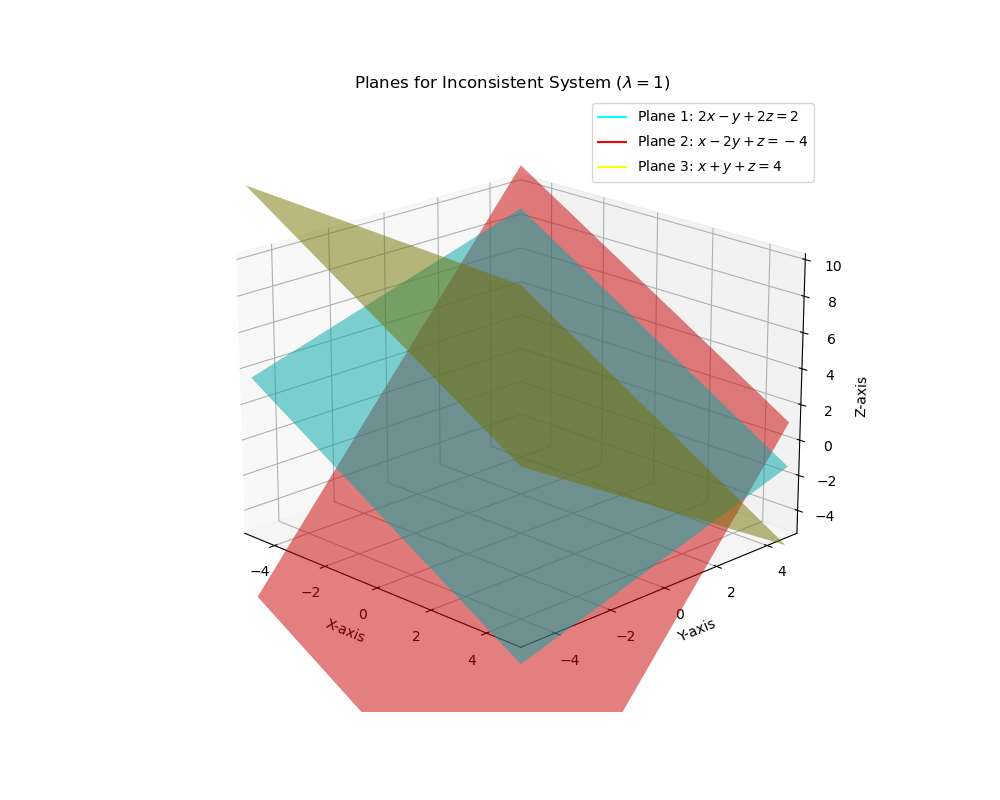
\includegraphics[width=\columnwidth, height=0.8\textheight, keepaspectratio]{figs/figure1.png}
        \end{center}
    \end{frame}
    
    \end{document}